

\documentclass{beamer}

%-- coding: UTF-8 --
\usepackage[UTF8]{ctex}
\usepackage{color}
\usepackage{caption}
\usepackage{graphicx}
\usepackage{subfigure}
%\usetheme{EastLansing}
%\usetheme{CambridgeUS}
\useinnertheme{rounded}
%\usecolortheme{rose}
\usecolortheme{spruce}

\title{从零开始学数模}
\subtitle{数学建模协会新生交流会}
\author{段晨光}
\institute{数学与统计学院2016级信息与计算科学专业}
\date{\today}

\begin{document}
\begin{frame}
	\titlepage
\end{frame}

\section*{Outline}
\begin{frame}
	\frametitle{Outline}
	\tableofcontents%[pausesections]
\end{frame}

\section{数学建模概论}
\section{入门篇}
	\subsection{线性代数中的数学模型}
	\subsection{高等数学中的数学模型}
	\subsection{概率论与数理统计中的数学模型}
	\subsection{大学物理中的数学模型}
	\subsection{MATLAB速成}
	\subsection{小结:从平时课程中学建模}
\section{进阶篇}
	\subsection{统计模型}
	\subsection{运筹学与优化模型}
	\subsection{微分方程模型}
	\subsection{数值计算}
	\subsection{其他高级模型}
	\subsection{小结:知其然更要知其所以然}
\section{数学建模实例}
\section{总结}	
	
\begin{frame}{数学建模概论}
各种各样的比赛:国赛,美赛,华中赛,五一赛,亚太数学建模(小美赛)……

各种各样的赛题:物理,生物,经济,社会……

受限的时间:3天

\textbf{应该学好数学,更应该学会数学建模。}

\textbf{才能让那些因为学数学而凋零的头发不白白牺牲。}

\end{frame}

\begin{frame}{入门篇}
- 学习熟悉MATLAB基本语法,可以利用MATLAB自带函数工具箱解决数学课程中的简单问题。

- 体会数学理论解决实际问题的思想,明确数学理论与实际问题之间的异同。

\end{frame}


\begin{frame}{入门篇}{线性代数中的数学模型}
\begin{block}{线性代数基础知识}

\textbf{向量}:从三维到n维;行向量,列向量,向量的内积

\textbf{矩阵}:什么是矩阵,矩阵有什么运算,从向量内积到矩阵乘法

\textbf{线性方程组}:线性方程组与矩阵

\textbf{特征值与特征向量}:什么是特征值,什么特征向量?有什么数学或实际意义?

\textbf{矩阵分解}:几种常用的矩阵分解?SVD分解
\end{block}
\end{frame}

\begin{frame}{入门篇}{线性代数中的数学模型举例}
\begin{block}{模型一:离散动力系统模型}

地理学家对人口的迁移很感兴趣。现考虑人口在A城市市区与它郊区之间的迁移的简单模型。

人口学统计表明,该地区每年有5\%城市人口流出到郊区,3\%的郊区人口流入市区。

假设不考虑人口出生与死亡,迁移率保持常数不变,不考虑城市外的人口与城市,t = 0 时,市区人口与郊区人口比例为3:2。

试建立模型,描述未来人口变化。
\end{block}
\end{frame}

\begin{frame}{入门篇}{线性代数中的数学模型举例}
\begin{block}{模型二:离散动力系统模型长期行为的稳定性}
在模型一中,当该系统长期运行,将会出现什么情况?是否与系统初始状态有关?
\end{block}
\end{frame}

\begin{frame}{入门篇}{线性代数中的数学模型举例——特征值与特征向量}
\begin{block}{模型三:斑点猫头鹰问题——离散动力系统稳定性讨论}
1990年,在利用太平洋西北部大面积森林问题上,北方的斑点猫头鹰成为争论的焦点。环境保护学家试图说服联邦政府,如果砍伐原始森林的行为得不到制止的话,猫头鹰将面临灭绝的危险;但木材行业辩解猫头鹰不会濒危。数学生态学家为此加快对猫头鹰的种群动力学研究。
\end{block}
\end{frame}

\begin{frame}{入门篇}{线性代数中的数学模型举例——特征值与特征向量}
猫头鹰的生命周期自然地分为三个阶段:幼年期(1岁以前)、半成年期(1~2岁)、成年期(2岁以后)。猫头鹰交配在半成年期和成年期,开始生育繁殖,可以活到20岁左右。

按照实际统计数据,在每一个阶段雌雄比接近1:1,从某一年到下一年中,新生幼年期猫头鹰为上一年猫头鹰数量的0.33倍,其中0.60的幼年雌猫头鹰得以生存,之后离开巢穴。砍伐森林之前,其中的0.50可以找到新的栖息地,但砍伐森林之后只有其中的0.30得以找到新的栖息地,进入半成年期,其他的在寻找过程失踪。0.71的半成年猫头鹰和0.94的成年猫头鹰将被记入成年猫头鹰。

试建立模型分析砍伐前后斑点猫头鹰的种群演变情况,并预测是否会灭绝。

\footnotesize 拓展阅读:
\emph{《线性代数及其应用》David C.Lay,机械工业出版社}.
\end{frame}

\begin{frame}{入门篇}{线性代数中的数学模型举例}
\begin{block}{模型四:基于SVD分解的图像压缩}
算法:

设有一幅图像对应的矩阵$A$(大小为$m\times n$,一般为灰度矩阵),对$A_k$进行奇异值分解,得$A_k=U{\Sigma}V^T$,其中$\Sigma$为奇异值矩阵,$U$,$V$均为正交矩阵。基于矩阵奇异值分解的数字图像压缩算法,其目标就是利用更小的储存空间尽可能多地储存图片的信息。奇异值分解后,矩阵$\Sigma$中对角元即特征值且从上到下降序排列。这里定义一个描述压缩程度的参数$\alpha$,称为压缩因子。压缩过程为选取$\Sigma$前部分项,剩余项置0,再将得到的$\hat{\Sigma}$与$U$和$V^T$相乘得到压缩后地图像。
\end{block}
\end{frame}

\begin{frame}{入门篇}{线性代数中的数学模型举例}
\begin{block}{模型五:基于SVD分解的数字水印嵌入算法}
算法:

{\color{blue} (1)水印嵌入}

设有一幅图像对应的矩阵$A$(大小为$m\times n$,一般为灰度矩阵),需要嵌入的水印对应矩阵$W$(大小为$m_1 \times n_1$),$A$的某一个大小为$m_1 \times n_1$的子块为$A_k$,其中,$m>m_1$,$n>n_1$。其步骤如下:

{\color{blue} Step1:}
对$A_k$进行奇异值分解,得$A_k=U{\Sigma}V^T$,其中$\Sigma$为奇异值矩阵,$U$,$V$均为正交矩阵。基于矩阵奇异值分解的数字水印算法,其目标就是将水印$W$嵌入到矩阵$\Sigma$中,这里定义一个描述水印嵌入程度的参数$\alpha$,称为强度因子,则水印嵌入过程表示为$\hat{\Sigma}=\Sigma+\alpha W$.

{\color{blue} Step2:}
对矩阵$\hat{\Sigma}$进行奇异值分解,得到$\hat{\Sigma}=\Sigma+\alpha W=U_1 {\Sigma}_1 {V_1}^T$,并令${\Sigma}_1$为嵌入水印后的图像$\hat{A_k}$的新奇异矩阵,由此可以得到嵌入水印后的图像子块$\hat{A_k}=U \Sigma_1 V^T$,更新原始图像,即完成水印嵌入。
\end{block}
\end{frame}

\begin{frame}{入门篇}{线性代数中的数学模型举例}

{\color{blue} (2)水印提取}

水印提取是上述水印嵌入的逆过程,假设我们得到的是受扰动的图像矩阵${A_k}^*$,对其进行奇异值分解${A_k}^*=U^* {\Sigma_1}^* V^*$,由此得到包含水印信息的奇异矩阵${\Sigma_1}^*$,然后利用水印嵌入时的矩阵$U_1$,$V_1$,得到$\hat{\Sigma}=U_1 {\Sigma_1}^* {V_1}^T$。由上述水印嵌入算法可得$W^*=\frac{1}{\alpha}(\hat{\Sigma}-\Sigma)$,从而得到水印的信息。

\begin{figure}
  \centering
  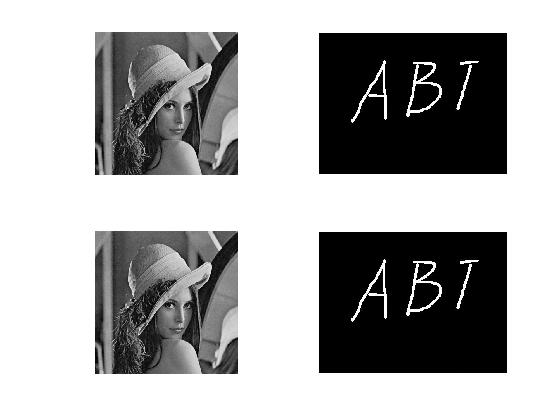
\includegraphics[width=.5\textwidth]{figure//fig01.png} 
  \caption{加水印前后对比} 
  \label{fig01} 
\end{figure}

\end{frame}

\begin{frame}{入门篇}{线性代数中的数学模型举例}

{\color{blue} 问题:}

1. 根据以上给出的算法,在MATLAB平台下编程实现,并用如下例图的方式显示结果(或建议设计GUI,图片和水印可以自行选定)。

2. 讨论如何选取子矩阵(位置)和参数,以得到好的水印嵌入和提取效果。

3. 若对图片进行攻击(旋转,压缩等),隐藏的信息是否可以提出?

\footnotesize 参考:
\emph{羿旭明老师《数学实验》课程}.

\end{frame}

\begin{frame}{入门篇}{线性代数中的数学模型举例}
\begin{block}{*模型六:基于SVD分解的主成分分析}
例如:通过正交变换将一组可能存在相关性的变量转换为一组线性不相关的变量,转换后的这组变量叫主成分。主成分分析可以消除变量之间的线性相关性,并且达到降维的目的。

\footnotesize 拓展阅读:
\emph{《应用多元统计分析》高惠璇,北京大学出版社}.
\end{block}
\end{frame}

\begin{frame}{入门篇}{高等数学中的数学模型}
\begin{block}{高等数学基础知识}

\textbf{极限}:什么是极限?什么是收敛?数学中的定义:$\epsilon-\delta$定义;实际应用中极限的理解(迭代收敛性的理解)?(hint:机器计算的有限性,结合模型二理解)

\textbf{导数}:什么是导数?导数的物理与几何意义?

\textbf{定积分}:什么是定积分?定积分的物理与几何意义?定积分的计算方式?

\textbf{常微分方程}:什么是常微分方程?常微分方程定解条件?常微分方程在几何和物理中的应用?常微分方程的求解?
\end{block}
\end{frame}

\begin{frame}{入门篇}{高等数学中的数学模型举例}
\begin{block}{模型七:非线性方程求解/函数交点}

Stewart平台是一个具有6个自由度的机器人,该平台可以极高的精度进行定位,最初由Dunlop Tire公司的Eric Gough在20世纪50年代发明,用于测试飞机的轮胎。现在,他的应用领域从非常大的飞机仿真器到精度十分重要的医药和手术应用。
\end{block}
\end{frame}

\begin{frame}{入门篇}{高等数学中的数学模型举例}

为了简化问题,仅考虑Stewart平台的二维版本。

\begin{figure}
  \centering
  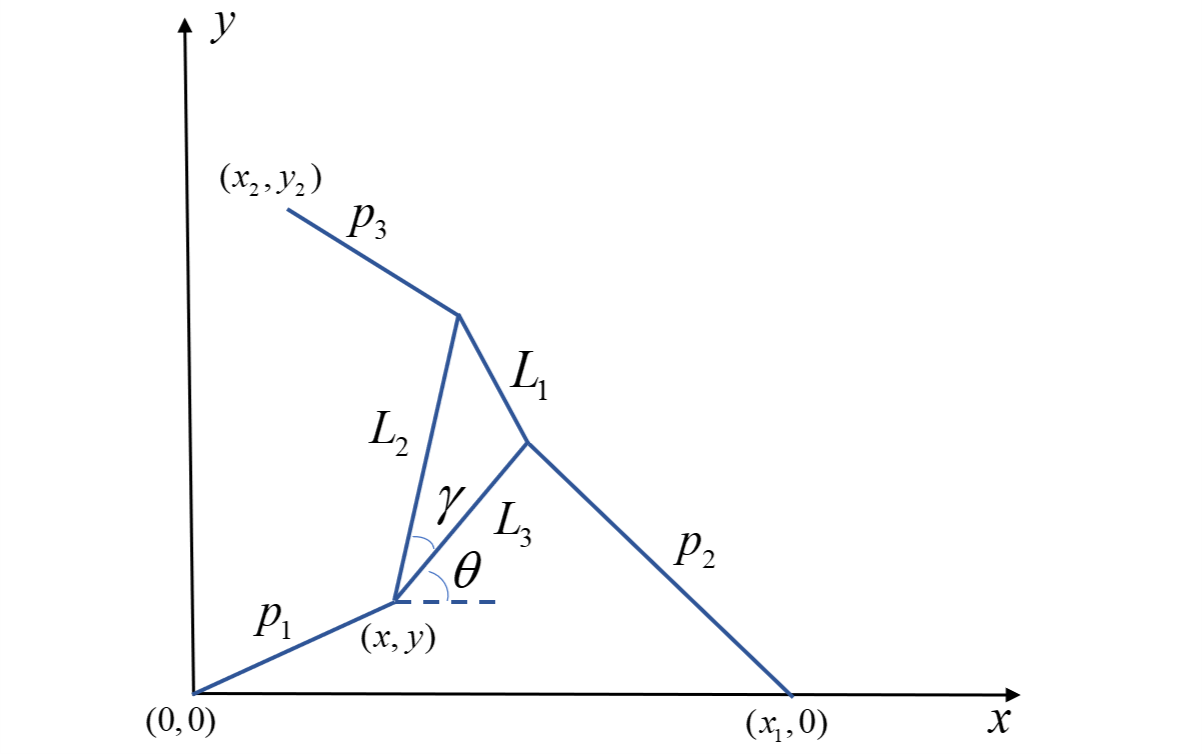
\includegraphics[width=.4\textwidth]{figure//fig02.png} 
  \caption{二维Stewart平台} 
  \label{fig02} 
\end{figure}

该控制器由三个支杆控制的平面上的一个三角形平台构成,如图所示。内部三角形表示平面Stewart平台,其对应的维度由三个长度$L_1$, $L_2$, $L_3$定义。令$\gamma$表示边$L_1$对应的角度,平台位置由三个长度$p_1$, $p_2$, $p_3$控制,对应三个支杆变化的长度。

试建立模型,要求在给定支杆长度的条件下,确定平台的位置和方向(控制器的前向运动学问题)。

\end{frame}

\begin{frame}{入门篇}{高等数学中的数学模型举例}
\begin{block}{模型八:油罐刻度的标定}
在石油的生产地和加工厂,为了储存原油,经常使用大量的储油罐.油罐的外形为一个圆柱体和两个圆锥体的组合,上端有一注油孔,如图所示。由于经常注油和取油,有时很难知道油罐中剩油的数量.这给现有储油量的统计带来很大的麻烦.显然,将剩油取出计量是不现实的.

\begin{figure}
  \centering
  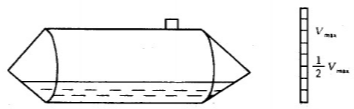
\includegraphics[width=.6\textwidth]{figure//fig03.png} 
  \caption{二维Stewart平台} 
  \label{fig03} 
\end{figure}

\end{block}
\end{frame}

\begin{frame}{入门篇}{高等数学中的数学模型举例}

试建立模型,设计一个精细的标尺:工人只需将该尺垂直插入使尺端至油罐的最底部,就可以根据标尺上的油痕位置的刻度获知剩油量的多少。这是一个来自油田的问题。

\footnotesize 拓展阅读:
\emph{油罐标尺刻度的设计.ppt}

\emph{国赛2010A题}.

\end{frame}

\begin{frame}{入门篇}{高等数学中的数学模型举例}
\begin{block}{模型九:常微分方程——人口模型}
对比离散动力系统模型,在方程导出、求解、稳定性分析上有对称结论。

\footnotesize 拓展阅读:
\emph{中国人口增长模型(国赛2007A题)}.
\end{block}
\begin{block}{模型十:常微分方程——传染病模型}
\footnotesize 拓展阅读:
\emph{SARS传染问题(国赛2003A题)}.

\footnotesize 拓展阅读:
\emph{罗壮初老师《数学建模中的微分方程模型》}.
\end{block}
\end{frame}

\begin{frame}{入门篇}{高等数学中的数学模型举例}
\begin{block}{*模型十一:函数极值——最小二乘和GPS}

\footnotesize 拓展阅读:
\emph{《数值分析》Timothy Sauer,机械工业出版社}.

\end{block}
\end{frame}

\begin{frame}{入门篇}{高等数学中的数学模型举例}
\begin{block}{模型十二:函数极值——分子形态预测}
1953年发现的DNA双螺旋结构为人类了解基因调控生命活动打开全新的窗口。但是直至今天,储存其中的信息仍有待人类翻译。

氨基酸折叠生成功能蛋白的关键依赖于Van der Waals力。在原子聚类模型中这些力使用Lennard-Jones势能进行建模,并在最小化能量的框架下进行研究。

当前预测蛋白质构成的一种方法是求氨基酸的完整构造的最小势能值,通过Lennard-Jones势能建立Van der Waals力
$$U(r)=\frac{1}{r^{12}}-\frac{2}{r^6}$$
其中$r$为两个原子之间距离。
\end{block}
\end{frame}


\begin{frame}{入门篇}{高等数学中的数学模型举例}
对于一族原子,他们的位置为$\{(x_i,y_i,z_i)\}^n_{i=1}$

则问题转换为
$$min \sum\limits_{i<j}(\frac{1}{r_{ij}^{12}}-\frac{2}{r_{ij}^6})$$
\end{frame}


\begin{frame}{入门篇}{大学物理中的数学模型举例}
\begin{block}{模型十三:带电粒子在非匀强磁场中的运动规律}
一非匀强磁场$B$沿着$z$方向,大小与$z$成正比:$B = Kzk$,$K$为比例系数。一质量为$m$,电量为$q$的带电粒子以初速度$v_0$从坐标原点射入磁场,初速度方向在$Oxz$平面内,与$z$方向的夹角为$\theta$,如图所示。
\begin{figure}
  \centering
  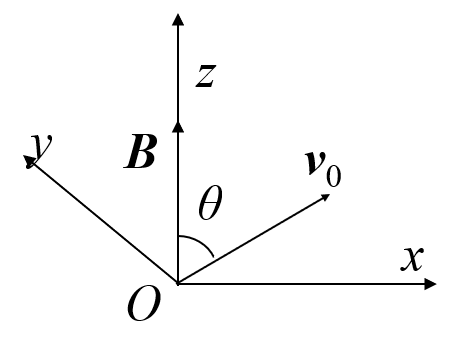
\includegraphics[width=.3\textwidth]{figure//fig04.png} 
  \caption{磁场示意图} 
  \label{fig04} 
\end{figure}
试建立模型描述粒子的运动轨迹。

\footnotesize 拓展阅读:
\emph{《MATLAB可视化大学物理学》周群益,清华大学出版社}.
\end{block}
\end{frame}

\begin{frame}{入门篇}{概率论与数理统计中的数学模型举例}
\begin{block}{模型十四:随机模拟——排队模型}

\footnotesize 拓展阅读:
\emph{《数学建模》Frank R. Giordano,机械工业出版社}.
\end{block}

\begin{block}{*模型十五:随机模拟——Black-Scholes期权定价模型}

\footnotesize 拓展阅读:
\emph{《数值分析》Timothy Sauer,机械工业出版社}.
\end{block}
\end{frame}

\begin{frame}{入门篇}{概率论与数理统计中的数学模型举例}
\begin{block}{模型十六:一元线性回归模型}
近 10 年来,某市社会商品零售总额与职工工资总额(单位:亿元)的数据见表,请建立社会商品零售总额与职工工资总额数据的回归模型。

\begin{table}[h]
\centering
\resizebox{0.9\hsize}{!}{
\begin{tabular}{|c|c|c|c|c|c|c|c|c|}
\hline
职工工资总额&23.8&27.6&31.6&32.4&33.7&34.9&42.3&52.8\\
\hline
商品零售总额&41.4&51.8&61.7&67.9&68.7&77.5&95.7&137.4\\
\hline
\end{tabular}
}
\caption{数据}
\label{table1}
\end{table}

\end{block}
\end{frame}

\begin{frame}{入门篇}{概率论与数理统计中的数学模型举例}
\begin{block}{模型十七:一元非线性回归模型}
为了解百货商店销售额与流通率(这是反映商业活动的一个质量指标,指每元商品流转额所分摊的流通费用)之间的关系,收集了九个商店的有关数据,见表。请建立它们关系的数学模型。

\begin{table}[h]
\centering
\resizebox{0.9\hsize}{!}{
\begin{tabular}{|c|c|c|c|c|c|c|c|c|c|}
\hline
销售总额(万元)&1.5&4.5&7.5&10.5&13.5&16.5&19.5&22.5&25.5\\
\hline
流通费率(\%)&7.0&4.8&3.6&3.1&2.7&2.5&2.4&2.3&2.2\\
\hline
\end{tabular}
}
\caption{数据}
\label{table2}
\end{table}

\end{block}
\end{frame}

\begin{frame}{入门篇}{推荐书目}
《数学建模》Frank R. Giordano,机械工业出版社

《数学建模方法与分析》Mark M. Meerschaert,机械工业出版社

\end{frame}

\begin{frame}{入门篇}{MATLAB速成}
\begin{block}{如何提高 MATLAB 编程水平}

MATLAB本身很简单,不存在壁垒,最大的问题是在没有树立正确的 MATLAB 使用理念,没有树立对 MATLAB使用的信心。这是因为在学习 MATLAB 的时候,一直机械地、被动地学习知识,而没有掌握技巧去搜索知识、运用知识。如果掌握正确的MATLAB使用方法,只要掌握些小技巧, 在半小时内就可以很快地变成 MATLAB 高手了,高手的区别就只在一点,就是一直有自己的编程思路,需要什么知识就是学习什么知识, 然后继续按照自己的思路编程,虽然在过程中,要不断学习,但最高效,也最容易建立的对 MATLAB 的使用信心。
\end{block}
\end{frame}

\begin{frame}{入门篇}{MATLAB速成}
\begin{block}{正确且高效的 MATLAB 编程理念就是以问题为中心的主动编程}


而以问题为中心的主动编程,则是先找到问题的解决步骤,然后在 MATLAB 中一步一步地去实现,在每步实现的过程中,遇到问题后,如果是需要知识就是查询知识(互联网时代查询知识还是很容易的),然后定位到方法,再根据方法,查询到 MATLAB 中的对应函数,查看函数的用法后,回到程序继续解决问题。通过这样的方式,逐步解决整个问题。在这个过程中,知识的获取都是为了解决问题的,也就是说每次学习的目标都是非常明确的,学完之后的应用更会强化对知识的理解和掌握,这样即学即用的学习方式是最有效的。

\end{block}
\end{frame}

\begin{frame}{入门篇}{MATLAB速成}
\begin{block}{好的编程一定以清晰的算法为前提}

整个建模过程中,清晰的模型和确定的算法是编程的必要条件。在“纸”上的功夫做足了,算法清晰了,再去碰键盘。最好养成画程序框图或者写伪代码的好习惯。而且这是算法改进的依据,毕竟算法的可读性远大于代码。

\end{block}
\end{frame}

\begin{frame}{入门篇}{MATLAB速成}
\begin{block}{提升能力的最快方式是比较自己和优秀作品之间的差距}

在这一方面,MATLAB作为商业软件,具有丰富的官方示例和完善的官方社区,里面有全球的MATLAB Coder相互讨论交流。
\end{block}
\end{frame}

\begin{frame}{入门篇}{MATLAB速成}
\begin{block}{如何快速提高 MATLAB 数学建模实战水平?}
{\color{blue} 第一部分:} 了解MATLAB的基本用法, 包括几个常用的命令, 如何获取帮助, 脚本结构, 程序的分节与注释, 矩阵的基本操作, 快捷绘图方式;熟悉MATLAB的程序结构,编程模式, 能自由地创建和引用函数(包括匿名函数)。

{\color{blue} 第二部分:} 利用MATLAB解决数学问题,包括辅助数学理解与学习,体会数学应用的想法与流程,提高从实际问题到数学问题的转化能力。

\end{block}
\end{frame}


\begin{frame}{入门篇}{MATLAB速成}
Documents: getstart.pdf

- 快速开始

- 语言基础

- 线性代数

- 可视化

- 控制流

- 函数

Website: https://ww2.mathworks.cn/

- Toolbox

- Documents

- Examples
\end{frame}



\begin{frame}{入门篇}{线性代数中的数学模型举例}
\begin{block}{模型一:离散动力系统模型}

地理学家对人口的迁移很感兴趣。现考虑人口在A城市市区与它郊区之间的迁移的简单模型。

人口学统计表明,该地区每年有5\%城市人口流出到郊区,3\%的郊区人口流入市区。

假设不考虑人口出生与死亡,迁移率保持常数不变,不考虑城市外的人口与城市,t = 0 时,市区人口与郊区人口比例为3:2。

试建立模型,描述未来人口变化。
\end{block}
\end{frame}

\begin{frame}{入门篇}{线性代数中的数学模型举例}
\begin{block}{模型二:离散动力系统模型长期行为的稳定性}
在模型一中,当该系统长期运行,将会出现什么情况?是否与系统初始状态有关?
\end{block}
\end{frame}

\begin{frame}{入门篇}{线性代数中的数学模型举例——特征值与特征向量}
\begin{block}{模型三:斑点猫头鹰问题——离散动力系统稳定性讨论}
1990年,在利用太平洋西北部大面积森林问题上,北方的斑点猫头鹰成为争论的焦点。环境保护学家试图说服联邦政府,如果砍伐原始森林的行为得不到制止的话,猫头鹰将面临灭绝的危险;但木材行业辩解猫头鹰不会濒危。数学生态学家为此加快对猫头鹰的种群动力学研究。
\end{block}
\end{frame}

\begin{frame}{入门篇}{线性代数中的数学模型举例——特征值与特征向量}
猫头鹰的生命周期自然地分为三个阶段:幼年期(1岁以前)、半成年期(1~2岁)、成年期(2岁以后)。猫头鹰交配在半成年期和成年期,开始生育繁殖,可以活到20岁左右。

按照实际统计数据,在每一个阶段雌雄比接近1:1,从某一年到下一年中,新生幼年期猫头鹰为上一年猫头鹰数量的0.33倍,其中0.60的幼年雌猫头鹰得以生存,之后离开巢穴。砍伐森林之前,其中的0.50可以找到新的栖息地,但砍伐森林之后只有其中的0.30得以找到新的栖息地,进入半成年期,其他的在寻找过程失踪。0.71的半成年猫头鹰和0.94的成年猫头鹰将被记入成年猫头鹰。

试建立模型分析砍伐前后斑点猫头鹰的种群演变情况,并预测是否会灭绝。

\footnotesize 拓展阅读:
\emph{《线性代数及其应用》David C.Lay,机械工业出版社}.
\end{frame}

\begin{frame}{入门篇}{线性代数中的数学模型举例}
\begin{block}{模型四:基于SVD分解的图像压缩}
算法:

设有一幅图像对应的矩阵$A$(大小为$m\times n$,一般为灰度矩阵),对$A_k$进行奇异值分解,得$A_k=U{\Sigma}V^T$,其中$\Sigma$为奇异值矩阵,$U$,$V$均为正交矩阵。基于矩阵奇异值分解的数字图像压缩算法,其目标就是利用更小的储存空间尽可能多地储存图片的信息。奇异值分解后,矩阵$\Sigma$中对角元即特征值且从上到下降序排列。这里定义一个描述压缩程度的参数$\alpha$,称为压缩因子。压缩过程为选取$\Sigma$前部分项,剩余项置0,再将得到的$\hat{\Sigma}$与$U$和$V^T$相乘得到压缩后地图像。
\end{block}
\end{frame}

\begin{frame}{入门篇}{线性代数中的数学模型举例}
\begin{block}{模型五:基于SVD分解的数字水印嵌入算法}
算法:

{\color{blue} (1)水印嵌入}

设有一幅图像对应的矩阵$A$(大小为$m\times n$,一般为灰度矩阵),需要嵌入的水印对应矩阵$W$(大小为$m_1 \times n_1$),$A$的某一个大小为$m_1 \times n_1$的子块为$A_k$,其中,$m>m_1$,$n>n_1$。其步骤如下:

{\color{blue} Step1:}
对$A_k$进行奇异值分解,得$A_k=U{\Sigma}V^T$,其中$\Sigma$为奇异值矩阵,$U$,$V$均为正交矩阵。基于矩阵奇异值分解的数字水印算法,其目标就是将水印$W$嵌入到矩阵$\Sigma$中,这里定义一个描述水印嵌入程度的参数$\alpha$,称为强度因子,则水印嵌入过程表示为$\hat{\Sigma}=\Sigma+\alpha W$.

{\color{blue} Step2:}
对矩阵$\hat{\Sigma}$进行奇异值分解,得到$\hat{\Sigma}=\Sigma+\alpha W=U_1 {\Sigma}_1 {V_1}^T$,并令${\Sigma}_1$为嵌入水印后的图像$\hat{A_k}$的新奇异矩阵,由此可以得到嵌入水印后的图像子块$\hat{A_k}=U \Sigma_1 V^T$,更新原始图像,即完成水印嵌入。
\end{block}
\end{frame}

\begin{frame}{入门篇}{线性代数中的数学模型举例}

{\color{blue} (2)水印提取}

水印提取是上述水印嵌入的逆过程,假设我们得到的是受扰动的图像矩阵${A_k}^*$,对其进行奇异值分解${A_k}^*=U^* {\Sigma_1}^* V^*$,由此得到包含水印信息的奇异矩阵${\Sigma_1}^*$,然后利用水印嵌入时的矩阵$U_1$,$V_1$,得到$\hat{\Sigma}=U_1 {\Sigma_1}^* {V_1}^T$。由上述水印嵌入算法可得$W^*=\frac{1}{\alpha}(\hat{\Sigma}-\Sigma)$,从而得到水印的信息。

\begin{figure}
  \centering
  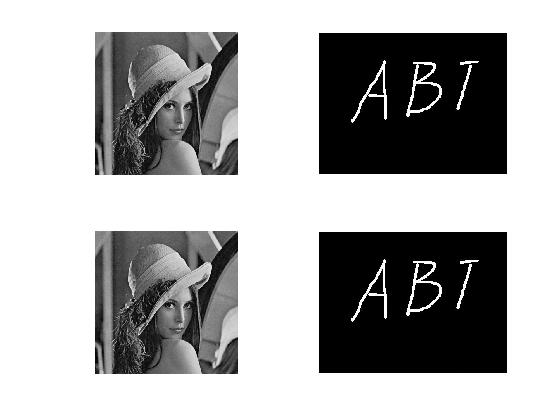
\includegraphics[width=.5\textwidth]{figure//fig01.png} 
  \caption{加水印前后对比} 
  \label{fig01} 
\end{figure}

\end{frame}

\begin{frame}{入门篇}{线性代数中的数学模型举例}

{\color{blue} 问题:}

1. 根据以上给出的算法,在MATLAB平台下编程实现,并用如下例图的方式显示结果(或建议设计GUI,图片和水印可以自行选定)。

2. 讨论如何选取子矩阵(位置)和参数,以得到好的水印嵌入和提取效果。

3. 若对图片进行攻击(旋转,压缩等),隐藏的信息是否可以提出?

\footnotesize 参考:
\emph{羿旭明老师《数学实验》课程}.

\end{frame}


\begin{frame}{入门篇}{高等数学中的数学模型举例}
\begin{block}{模型十二:函数极值——分子形态预测}
1953年发现的DNA双螺旋结构为人类了解基因调控生命活动打开全新的窗口。但是直至今天,储存其中的信息仍有待人类翻译。

氨基酸折叠生成功能蛋白的关键依赖于Van der Waals力。在原子聚类模型中这些力使用Lennard-Jones势能进行建模,并在最小化能量的框架下进行研究。

当前预测蛋白质构成的一种方法是求氨基酸的完整构造的最小势能值,通过Lennard-Jones势能建立Van der Waals力
$$U(r)=\frac{1}{r^{12}}-\frac{2}{r^6}$$
其中$r$为两个原子之间距离。
\end{block}
\end{frame}


\begin{frame}{入门篇}{高等数学中的数学模型举例}
对于一族原子,他们的位置为$\{(x_i,y_i,z_i)\}^n_{i=1}$

则问题转换为
$$min \sum\limits_{i<j}(\frac{1}{r_{ij}^{12}}-\frac{2}{r_{ij}^6})$$
\end{frame}


\begin{frame}{入门篇}{大学物理中的数学模型举例}
\begin{block}{模型十三:带电粒子在非匀强磁场中的运动规律}
一非匀强磁场$B$沿着$z$方向,大小与$z$成正比:$B = Kzk$,$K$为比例系数。一质量为$m$,电量为$q$的带电粒子以初速度$v_0$从坐标原点射入磁场,初速度方向在$Oxz$平面内,与$z$方向的夹角为$\theta$,如图所示。
\begin{figure}
  \centering
  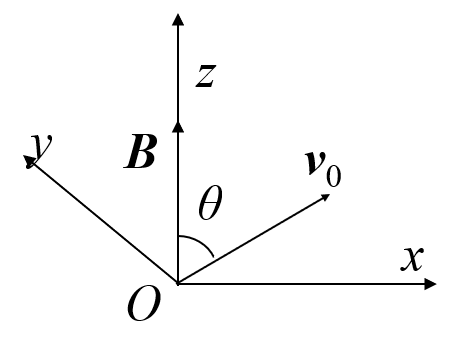
\includegraphics[width=.3\textwidth]{figure//fig04.png} 
  \caption{磁场示意图} 
  \label{fig04} 
\end{figure}
试建立模型描述粒子的运动轨迹。

\footnotesize 拓展阅读:
\emph{《MATLAB可视化大学物理学》周群益,清华大学出版社}.
\end{block}
\end{frame}

\begin{frame}{入门篇}{概率论与数理统计中的数学模型举例}
\begin{block}{模型十六:一元线性回归模型}
近 10 年来,某市社会商品零售总额与职工工资总额(单位:亿元)的数据见表,请建立社会商品零售总额与职工工资总额数据的回归模型。

\begin{table}[h]
\centering
\resizebox{0.9\hsize}{!}{
\begin{tabular}{|c|c|c|c|c|c|c|c|c|}
\hline
职工工资总额&23.8&27.6&31.6&32.4&33.7&34.9&42.3&52.8\\
\hline
商品零售总额&41.4&51.8&61.7&67.9&68.7&77.5&95.7&137.4\\
\hline
\end{tabular}
}
\caption{数据}
\label{table1}
\end{table}

\end{block}
\end{frame}

\begin{frame}{入门篇}{概率论与数理统计中的数学模型举例}
\begin{block}{模型十七:一元非线性回归模型}
为了解百货商店销售额与流通率(这是反映商业活动的一个质量指标,指每元商品流转额所分摊的流通费用)之间的关系,收集了九个商店的有关数据,见表。请建立它们关系的数学模型。

\begin{table}[h]
\centering
\resizebox{0.9\hsize}{!}{
\begin{tabular}{|c|c|c|c|c|c|c|c|c|c|}
\hline
销售总额(万元)&1.5&4.5&7.5&10.5&13.5&16.5&19.5&22.5&25.5\\
\hline
流通费率(\%)&7.0&4.8&3.6&3.1&2.7&2.5&2.4&2.3&2.2\\
\hline
\end{tabular}
}
\caption{数据}
\label{table2}
\end{table}

\end{block}
\end{frame}

\begin{frame}{入门篇}{小结:从平时课程中学建模}

《线性代数及其应用》David C. Lay,机械工业出版社

《数学建模》Frank R. Giordano,机械工业出版社

《数学建模方法与分析》Mark M. Meerschaert,机械工业出版社

\end{frame}

\begin{frame}{进阶篇}
- 学习更深入系统的数学理论

- 学习总结经典数学模型

- 能够熟练掌握MATLAB的使用,并对于常见问题,可以自行编写程序实现
\end{frame}

\begin{frame}{进阶篇}{统计建模}
\begin{block}{多元统计分析}
-多元回归分析

-方差分析

-判别分析

-聚类分析

-主成分分析

-因子分析

-典型相关性分析
\end{block}
\begin{block}{其他统计建模方法}
统计模拟

时间序列分析

……
\end{block}


\footnotesize Remark:不建议在不熟悉内容的情况下学习一门新的语言,易分散精力。

\footnotesize 拓展阅读:
\emph{《统计建模与R软件》薛毅,邓爱姣老师数模课件}.
\end{frame}

\begin{frame}{进阶篇}{运筹学与优化问题}
线性规划模型

整数规划模型

非线性规划问题

概率与运筹学结合

动态规划

图论中的规划问题

……


\footnotesize Remark:不建议在不熟悉内容的情况下学习一门新的语言,易分散精力。

\footnotesize 拓展阅读:
\emph{《优化建模与LINGO软件》薛毅,《运筹学》,清华大学出版社}.
\end{frame}


\begin{frame}{进阶篇}{微分方程问题}


\begin{block}{常微分方程}

人口模型

单摆模型

……
\end{block}

\begin{block}{偏微分方程}

弦振动模型,膜振动模型

热传导模型,扩散模型

……
\end{block}


\footnotesize Remark:微分方程求解,微分方程适定性问题建议了解

\end{frame}

\begin{frame}{进阶篇}{数值计算}

数值线性代数:直接法,迭代法

非线性方程求解——二分法,牛顿法

函数插值,逼近——多项式插值,样条插值

数值积分

微分方程数值解——常微分方程,偏微分方程

数值最优化(传统算法与启发式算法):基于导数的优化算法,搜索优化算法,模拟退火算法,遗传算法……

\footnotesize 拓展阅读:
\emph{《数值分析》Timothy Sauer,机械工业出版社}.
\end{frame}

\begin{frame}{进阶篇}{其他高级模型}

《数学模型》姜启源:博弈论,评价模型……

机器学习与神经网络:回归,分类,拟合——用好工具箱

\end{frame}

\begin{frame}{进阶篇}{小结:知其然更要知其所以然}

使用MATLAB完成基本的数学操作,并对“程式”以外的问题可以自行设计算法,编写程序,分析结果。

特别的,对常用的数值计算与数值优化方法要了解算法细节,尽可能自行实现。

此外,在实际建模中往往会将建模、代码、写作分开,但是学习训练过程,不可偏废任一项,“全面”是数学建模的关键。

\end{frame}

\begin{frame}{数学建模实例}{数学建模思想}
\begin{block}{转化思想}
问题拆分

未知转化为已知
\end{block}
\end{frame}


\begin{frame}{数学建模实例}{数学建模思想}
\begin{block}{类比思想}
事物背后的数学原理的相似性
\begin{figure}
\subfigure{\label{fig:subfig:a}
  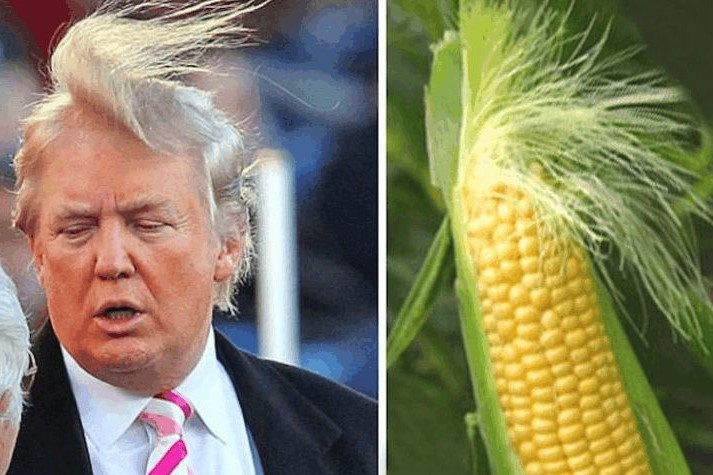
\includegraphics[width=.2\textwidth]{figure//fig05.png}}
\subfigure{\label{fig:subfig:b}
  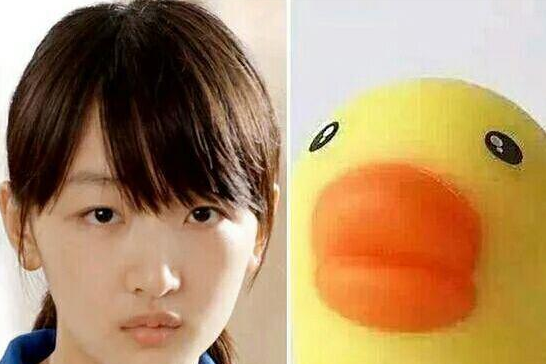
\includegraphics[width=.2\textwidth]{figure//fig06.png}}
\subfigure{\label{fig:subfig:c}
  
\includegraphics[width=.2\textwidth]{figure//fig07.png}}
\subfigure{\label{fig:subfig:d}
  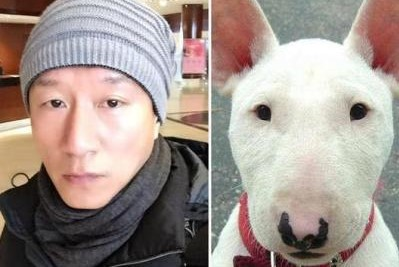
\includegraphics[width=.2\textwidth]{figure//fig08.png}}
\subfigure{\label{fig:subfig:e}
  
\includegraphics[width=.2\textwidth]{figure//fig09.png}}
\label{fig:subfig} 
\end{figure}
\end{block}
\end{frame}



\begin{frame}{数学建模实例}{打车问题}
\begin{block}{2015国赛B题 “互联网+”时代的出租车资源配置}

出租车是市民出行的重要交通工具之一,“打车难”是人们关注的一个社会热点问题。随着“互联网+”时代的到来,有多家公司依托移动互联网建立了打车软件服务平台,实现了乘客与出租车司机之间的信息互通,同时推出了多种出租车的补贴方案。
请你们搜集相关数据,建立数学模型研究如下问题:

(1) 试建立合理的指标,并分析不同时空出租车资源的“供求匹配”程度。

(2) 分析各公司的出租车补贴方案是否对“缓解打车难”有帮助?

(3) 如果要创建一个新的打车软件服务平台,你们将设计什么样的补贴方案,并论证其合理性。

\footnotesize 拓展阅读:
\emph{国赛2015B题MATLAB创新奖.pdf}
\end{block}
\end{frame}

\begin{frame}{数学建模实例}{天体运动与轨道力学}
此处,我们仅考虑一个平面内的运动。对于两个天体的系统,这是平凡的;对于三个天体的运动,我们对系统添加约束,将其限制在平面内。
$$F = \frac{GMm}{r^2}$$
\end{frame}

\begin{frame}{数学建模实例}{天体运动与轨道力学}
\begin{block}{单体运动}
考虑两个天体$A$,$B$的系统,其中$A$的质量记为$M$,$B$的质量记为$m$,并且有$m \ll M$,例如一个小的行星围绕一个大的恒星运动的情况。此时,不妨假设恒星位置固定。
由牛顿第二定律得到两个二阶方程
$$m\ddot{x}=-\frac{GMmx}{(x^2+y^2)^{3/2}}$$
$$m\ddot{y}=-\frac{GMmy}{(x^2+y^2)^{3/2}}$$
\end{block}
\end{frame}

\begin{frame}{数学建模实例}{天体运动与轨道力学}
引入变量:$v_x=\dot{x}$,$v_y=\dot{y}$将两个二阶方程化为四个一阶方程组:
$$
\left \{
\begin{aligned}
\dot{x}   & =  v_x \\
\dot{v_x} & =  -\frac{GMx}{(x^2+y^2)^{3/2}} \\
\dot{y}   & =  v_y \\
\dot{v_y} & =  -\frac{GMy}{(x^2+y^2)^{3/2}} 
\end{aligned}
\right. 
$$

\end{frame}


\begin{frame}{数学建模实例}{天体运动与轨道力学}
\begin{block}{二体运动}
若取消单体运动中的假设,认为两天体质量在同一量级,例如两恒星系统的运动。同样不考虑二者相互作用以外的受力。二体问题由8个方程构成系统,每个物体有四个方程,也是由牛顿第二定律得到。

例如,对第一个物体:
$$
\left \{
\begin{aligned}
\dot{x_1}   & =  v_{1x} \\
\dot{v_{1x}} & =  \frac{G{m_2}(x_2-x_1)}{((x_2-x_1)^2+(y_2-y_1)^2)^{3/2}} \\
\dot{y_1}   & =  v_{1y} \\
\dot{v_{1y}} & =  \frac{G{m_2}(y_2-y_1)}{((x_2-x_1)^2+(y_2-y_1)^2)^{3/2}} \\
\end{aligned}
\right. 
$$

\end{block}
\end{frame}

\begin{frame}{数学建模实例}{天体运动与轨道力学}
\begin{block}{三体运动}
三个物体在引力作用下相互作用的情形称为三体问题,它在科学史上占有重要位置。即使当所有运动被限制在一个平面(约束三体问题),长期轨道在本质上是可不预估的。1889年,瑞典和挪威国王Oscar二世悬赏证明太阳系的稳定性,Henri Poincare得到这一奖项,他证明了对于三个交互物体的运动现象,根本不可能证明稳定性。

非预测性来自于对初值条件的敏感依赖,即初始位置和速度的微小不确定导致在随后时间可能出现较大偏差。

\end{block}
\end{frame}

\begin{frame}{数学建模实例}{天体运动与轨道力学}
受限三体问题由12个方程构成系统,每个物体有四个方程,也是由牛顿第二定律得到。

例如,对第一个物体:

$$
\left \{
\begin{aligned}
\dot{x_1}   & =  v_{1x} \\
\dot{v_{1x}} & =  \frac{G{m_2}(x_2-x_1)}{((x_2-x_1)^2+(y_2-y_1)^2)^{3/2}}+\frac{G{m_3}(x_3-x_1)}{((x_3-x_1)^2+(y_3-y_1)^2)^{3/2}} \\
\dot{y_1}   & =  v_{1y} \\
\dot{v_{1y}} & =  \frac{G{m_2}(y_2-y_1)}{((x_2-x_1)^2+(y_2-y_1)^2)^{3/2}}+\frac{G{m_3}(y_3-y_1)}{((x_3-x_1)^2+(y_3-y_1)^2)^{3/2}} \\
\end{aligned}
\right. 
$$
\end{frame}

\begin{frame}{数学建模实例}{天体运动与轨道力学}
\begin{block}{模型分析}
误差一:欧拉法的不稳定性(数值方法带来的误差)

误差二:对初值条件的敏感依赖(问题本身的是病态的)
\end{block}
\end{frame}


\end{document}

















